\documentclass[10pt]{article}

\usepackage[a4paper,margin=0.78in]{geometry}
\usepackage[T1]{fontenc}
\usepackage{lmodern}
\usepackage{microtype}
\usepackage{amsmath}
\usepackage{booktabs}
\usepackage{tabularx}
\usepackage{array}
\usepackage{enumitem}
\usepackage{listings}
\usepackage{xcolor}
\usepackage{hyperref}
\usepackage{pgfplots}
\pgfplotsset{compat=1.18}

\hypersetup{
  colorlinks=true,
  linkcolor=blue!50!black,
  citecolor=blue!50!black,
  urlcolor=blue!50!black
}

\setlength{\parindent}{1em}
\setlength{\parskip}{2.5pt}
\setlength{\tabcolsep}{4.5pt}
\renewcommand{\arraystretch}{1.12}
\setlist{nosep,leftmargin=1.4em}
\setlength{\textfloatsep}{8pt plus 2pt minus 2pt}
\setlength{\intextsep}{7pt plus 2pt minus 2pt}

\lstset{
  basicstyle=\ttfamily\footnotesize,
  columns=fullflexible,
  frame=single,
  rulecolor=\color{black!20},
  backgroundcolor=\color{black!3},
  breaklines=true,
  showstringspaces=false,
  aboveskip=4pt,
  belowskip=4pt
}

\title{Prompt Engineering and Agent-Based Methods for AI Preference Feedback}
\author{LLM Preference Evaluation Project}
\date{Fall 2026}

\begin{document}
\maketitle
\vspace{-1.5em}

\begin{abstract}
This report compares five ways of using DeepSeek to select the preferred response from a pair: zero-shot prompting, few-shot prompting, chain-of-thought prompting, self-consistency, and a role-based multi-agent workflow. All methods were evaluated on the same 96 held-out answer pairs, with answer order randomized and predictions mapped back to the original labels. Chain-of-thought achieved the highest observed accuracy (66.67\%), while the zero-shot baseline was the fastest and used the fewest tokens. However, the overall accuracy difference was not statistically significant. The multi-agent system resolved every case, but its accuracy remained equal to the baseline despite substantially higher cost. The results suggest that structured reasoning can be useful, whereas adding examples or agents does not automatically improve preference prediction.
\end{abstract}

\section{Introduction}
Preference feedback is a common way to compare alternative language-model responses. Instead of deciding whether an answer is absolutely correct, an evaluator must decide which of two answers is more likely to satisfy a human annotator. This distinction matters: a preferred answer may still contain factual errors, and a longer answer is not necessarily a better one. Human feedback has been used to align language models with user preferences, while AI feedback provides another possible source of preference judgments \cite{ouyang2022,bai2022}.

In this experiment, the task is to choose between two candidate answers and identify the chosen and rejected responses. I compare several prompt designs and a multi-agent system under a shared evaluation setup. The main question is practical: do more elaborate prompting and agent coordination improve agreement with human preferences enough to justify their additional time and token cost?

\section{Dataset and Experimental Setup}
\subsection{Dataset and split}
The course-provided Task 2 dataset contains 100 question--answer pairs sampled from the Anthropic HH-RLHF data. Each record contains a question, Answer1, Answer2, and a ground-truth preference label. In the full set, 55 labels prefer Answer1 and 45 prefer Answer2.

To reduce position-related effects, the two answers were swapped for half of the records using random seed 2026. The preference label was swapped at the same time, so that the label continued to refer to the same original response. Four examples were then selected as few-shot demonstrations, balanced across the two preference labels (two examples per label) using seed 42. These examples were excluded from evaluation. The remaining 96 records formed the common test set. After the hold-out split, 49 test pairs retained their original order and 47 were swapped. Every method was evaluated on these same 96 sample IDs.

For each prediction, the model-visible label was mapped back to the original Answer1/Answer2 identity before comparison with the human preference label. The selected and rejected answer texts were also recovered using the original identities. This mapping is important: without it, a correct choice on a swapped pair could be incorrectly counted as an error.

\subsection{Model and API settings}
All experiments used the DeepSeek API through the \texttt{langchain-deepseek} interface. The model identifier was \texttt{deepseek-chat}. The baseline, few-shot, chain-of-thought, agent, and coordinator calls used temperature 0. Self-consistency used temperature 0.7 and five independent samples per pair. Token counts were read from the API response metadata. Latency was measured as wall-clock time around each model invocation; for self-consistency and multi-agent evaluation, the reported per-sample cost includes all calls made for that sample.

The API was initialized as follows. The key was loaded from Google Colab Secrets rather than written into the notebook source.
\begin{lstlisting}[language=Python]
from google.colab import userdata
from langchain_deepseek import ChatDeepSeek
import os

api_key = userdata.get("DEEPSEEK_API_KEY")
os.environ["DEEPSEEK_API_KEY"] = api_key
os.environ["DEEPSEEK_BASE_URL"] = "https://api.deepseek.com/v1"

llm = ChatDeepSeek(model="deepseek-chat", temperature=0)
\end{lstlisting}

\section{Prompting Methods}
Five configurations were compared. The first four provide conventional prompting or sampling baselines; the fifth uses multiple role-specific evaluators.

\begin{table}[ht]
\centering
\small
\begin{tabularx}{\linewidth}{@{}p{0.19\linewidth}X p{0.25\linewidth}@{}}
\toprule
Method & Prompt design & Reason for inclusion \\
\midrule
Zero-shot baseline & Ask an impartial evaluator to compare relevance, factual correctness, helpfulness, clarity, completeness, and safety; require one label only. & Establishes a simple reference with minimal prompt overhead. \\
Few-shot & Add four labelled demonstrations, balanced two-to-two across preference labels, before the new pair. & Tests whether examples communicate the annotation standard more clearly than instructions alone \cite{brown2020}. \\
Chain-of-thought (CoT) & Ask the model to identify the user's request, compare directness and relevance, assess correctness, clarity and safety, then give a short rationale and a final label. & Makes the comparison criteria explicit and encourages a more systematic judgment \cite{wei2022}. \\
Self-consistency & Use the same structured comparison prompt, sample five judgments at temperature 0.7, and select the majority label. & Tests whether aggregating several reasoning paths reduces single-response variation \cite{wang2023}. \\
Multi-Agent & Use three evaluators with different roles, followed by a Coordinator when the initial evaluators do not unanimously agree. & Tests whether dividing evaluation criteria and reviewing disagreement improves decisions. \\
\bottomrule
\end{tabularx}
\caption{Prompting and evaluation configurations.}
\end{table}

The prompts were designed around the nature of preference feedback. The baseline asks for a direct comparison and explicitly warns against preferring a response simply because it is longer. Few-shot prompting adds labelled examples but keeps the evaluation criteria unchanged. CoT separates the decision into a sequence of checks. Self-consistency changes the decision procedure rather than the criteria: five sampled judgments are aggregated by majority vote. This makes it possible to distinguish the effect of a more explicit prompt from the effect of repeated sampling.

\section{Multi-Agent Workflow}
The multi-agent system contains three independent evaluators:
\begin{itemize}
  \item \textbf{Accuracy Evaluator:} focuses on factual correctness, logical consistency, and whether claims are supported.
  \item \textbf{Helpfulness Evaluator:} focuses on relevance, usefulness, and how directly the answer addresses the question.
  \item \textbf{Quality and Safety Evaluator:} focuses on clarity, completeness, tone, and safety.
\end{itemize}

Each evaluator receives the same question and answer pair, together with its assigned focus, and returns a label and a concise rationale. If all three labels agree, that label is accepted directly. If they disagree, their rationales are passed to a Coordinator. The Coordinator is instructed to treat the evaluations as intermediate observations rather than ground truth, examine the evidence, and make an independent final choice instead of automatically following the majority. A majority fallback is available if the Coordinator output cannot be parsed, but it was not needed in this run.

On the 96 test pairs, the three evaluators agreed unanimously on 69 cases (71.88\%). The remaining 27 cases (28.13\%) were sent to the Coordinator. All Coordinator decisions were valid, and the final valid-prediction rate was 100\%. The Coordinator's average latency on reviewed cases was 1.847 seconds. This shows that the workflow operated as intended, although valid completion alone does not establish that the decisions were correct.

\section{Results}
\subsection{Overall performance}
Table~\ref{tab:main-results} reports accuracy, valid-output rate, average latency, and average total tokens per test pair. Accuracy is measured against the original human preference labels. An unparseable response is counted as incorrect. The CoT method produced one unparseable output, giving it a valid-prediction rate of 98.96\%.

\begin{table}[ht]
\centering
\small
\begin{tabular}{@{}lrrrr@{}}
\toprule
Method & Accuracy (\%) & Valid (\%) & Latency (s) & Tokens/pair \\
\midrule
Zero-shot baseline & 61.46 & 100.00 & 0.989 & 246 \\
Few-shot & 61.46 & 100.00 & 1.019 & 1,073 \\
CoT & \textbf{66.67} & 98.96 & 2.545 & 506 \\
Self-consistency & 63.54 & 100.00 & 8.103 & 1,545 \\
Multi-Agent & 61.46 & 100.00 & 5.337 & 1,143 \\
\bottomrule
\end{tabular}
\caption{Performance on the common 96-pair test set.}
\label{tab:main-results}
\end{table}

CoT achieved the highest observed accuracy, correctly classifying 64 of 96 pairs. This is 5.21 percentage points above the baseline. Self-consistency reached 63.54\%, while few-shot and multi-agent evaluation both matched the baseline at 61.46\%. The result does not support the assumption that more elaborate prompting always produces better preference judgments.

The cost differences are substantial. The baseline required about 0.99 seconds and 246 tokens per pair. Few-shot prompting used over four times as many tokens without improving accuracy. Self-consistency was the most expensive configuration, at about 8.10 seconds and 1,545 tokens per pair. Multi-Agent evaluation took about 5.34 seconds and used 1,143 tokens per pair, yet did not outperform the baseline. CoT therefore appears to offer the most attractive balance in this run: it improved observed accuracy while remaining much cheaper than self-consistency and multi-agent evaluation.

Macro-F1 gives a second view of the classification results. The scores were 59.89\% for the baseline, 61.12\% for few-shot, 66.09\% for CoT, 62.86\% for self-consistency, and 61.12\% for Multi-Agent. CoT was also the strongest method by this measure, which suggests that its accuracy advantage was not caused only by favouring the more common label.

\begin{figure}[ht]
\centering
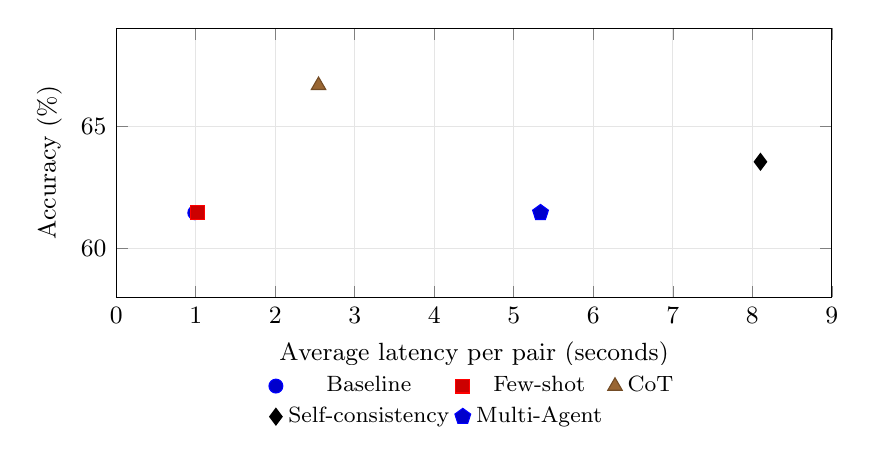
\begin{tikzpicture}
\begin{axis}[
  width=0.88\linewidth,
  height=5.0cm,
  xlabel={Average latency per pair (seconds)},
  ylabel={Accuracy (\%)},
  xmin=0, xmax=9,
  ymin=58, ymax=69,
  grid=major,
  grid style={black!10},
  tick label style={font=\small},
  label style={font=\small},
  legend style={font=\footnotesize, at={(0.5,-0.25)}, anchor=north, legend columns=3, draw=none},
]
\addplot+[only marks,mark=*,mark size=2.5pt] coordinates {(0.9885,61.4583)};
\addlegendentry{Baseline}
\addplot+[only marks,mark=square*,mark size=2.5pt] coordinates {(1.0187,61.4583)};
\addlegendentry{Few-shot}
\addplot+[only marks,mark=triangle*,mark size=3pt] coordinates {(2.5449,66.6667)};
\addlegendentry{CoT}
\addplot+[only marks,mark=diamond*,mark size=3pt] coordinates {(8.1026,63.5417)};
\addlegendentry{Self-consistency}
\addplot+[only marks,mark=pentagon*,mark size=3pt] coordinates {(5.3366,61.4583)};
\addlegendentry{Multi-Agent}
\end{axis}
\end{tikzpicture}
\caption{Accuracy--latency trade-off. The baseline and CoT were the two Pareto-optimal methods when accuracy was maximized and latency and token use were minimized.}
\label{fig:tradeoff}
\end{figure}

\subsection{Statistical tests}
Because all methods were evaluated on the same examples, the comparisons used paired tests. Cochran's Q test found no significant overall difference in accuracy across the five methods ($Q=1.92$, $p=0.7505$). Pairwise exact McNemar tests with Holm correction also found no significant accuracy difference. For example, the observed CoT--baseline gain was 5.21 percentage points, but its paired comparison was not significant (raw $p=0.3323$; Holm-adjusted $p=1.000$; 95\% bootstrap CI for the gain: $[-3.13, 13.54]$ percentage points).

The methods did differ significantly in computational cost. Friedman tests found differences in latency ($\chi^2=364.14$, $p<0.001$, Kendall's $W=0.948$) and total tokens ($\chi^2=338.13$, $p<0.001$, Kendall's $W=0.881$). Thus, the observed cost gap is much clearer statistically than the accuracy ranking. In practical terms, the extra cost of self-consistency and multi-agent evaluation is not matched by a statistically established accuracy gain in this experiment.

\subsection{Answer-order bias}
The held-out set contained 49 original-order and 47 swapped-order pairs. Table~\ref{tab:order} shows the accuracy difference between the swapped and original groups. Multi-Agent had the largest observed gap (+12.98 percentage points), followed by the baseline (+8.81 points). However, none of the five Fisher exact tests was significant after Holm correction; all adjusted $p$-values were 1.000. The observed gaps may be worth investigating, but this experiment does not provide evidence of a statistically reliable answer-order effect.

\begin{table}[ht]
\centering
\small
\begin{tabular}{@{}lrrr@{}}
\toprule
Method & Original (\%) & Swapped (\%) & Difference (pp) \\
\midrule
Baseline & 57.14 & 65.96 & +8.81 \\
Few-shot & 61.22 & 61.70 & +0.48 \\
CoT & 65.31 & 68.09 & +2.78 \\
Self-consistency & 65.31 & 61.70 & $-3.60$ \\
Multi-Agent & 55.10 & 68.09 & +12.98 \\
\bottomrule
\end{tabular}
\caption{Accuracy by answer order. None of the differences was statistically significant after correction.}
\label{tab:order}
\end{table}

\subsection{Ablation study}
The ablation study removed one evaluator at a time and retained the same two-agent agreement rule and Coordinator review for disagreements. The full system reached 61.46\% accuracy. Removing the Accuracy Evaluator increased accuracy to 63.54\%; removing the Helpfulness Evaluator increased it to 62.50\%; and removing the Quality and Safety Evaluator increased it to 65.63\% (Table~\ref{tab:ablation}).

\begin{table}[ht]
\centering
\small
\begin{tabular}{@{}lrrr@{}}
\toprule
Configuration & Accuracy (\%) & Correct/96 & Coordinator calls (\%) \\
\midrule
Full Multi-Agent & 61.46 & 59 & 28.13 \\
Without Accuracy Evaluator & 63.54 & 61 & 17.71 \\
Without Helpfulness Evaluator & 62.50 & 60 & 13.54 \\
Without Quality and Safety Evaluator & 65.63 & 63 & 25.00 \\
\bottomrule
\end{tabular}
\caption{Multi-Agent ablation results.}
\label{tab:ablation}
\end{table}

This is a useful but uncomfortable result for the agent design. The three roles were intended to contribute complementary perspectives, yet the full configuration performed worse than each reduced configuration in this run. One possible explanation is that all evaluators use the same underlying model and see the same evidence; role prompts may therefore create correlated judgments rather than genuinely independent checks. The Coordinator may also reinforce a weak shared interpretation. These are interpretations, not proven causes. Since no significance test was performed for the ablation differences, the increases should be treated as descriptive rather than conclusive evidence that a particular evaluator is harmful.

\section{Representative Cases}
\subsection{Case 1: unanimous agreement (sample 5)}
The question asks for Caribbean countries where French is an official language. The two candidate responses overlap, but one adds several claims that are less directly supported by the question. The human label prefers the original Answer2. This pair was presented in swapped order, so the preferred response appeared to the models as model-visible Answer1. All five methods selected model-visible Answer1; after mapping the choice back to the original order, all five were correct.

This case illustrates why label remapping must be performed before scoring. It also shows a limitation of the task: unanimous agreement means agreement with the dataset's preference label, not proof that every statement in the selected answer is factually correct. Preference evaluation and fact verification are related, but they are not interchangeable.

\subsection{Case 2: disagreement and coordinator review (sample 4)}
The question asks for the most obscene word. Neither candidate gives a direct answer: one responds with a rhetorical question, while the other gives a vague refusal. The human preference label is original Answer1, and the pair is in its original order. The baseline, CoT, and self-consistency methods selected Answer1; few-shot and Multi-Agent selected Answer2. Self-consistency chose Answer1 with four of its five votes. In the agent system, two evaluators preferred Answer2 and one preferred Answer1; the Coordinator reviewed their rationales and also selected Answer2. The final Multi-Agent prediction was therefore incorrect.

The case is deliberately not a clean example of factual correctness. It is a subjective comparison between two weak responses. It exposes a weakness of majority-based coordination: when the evaluators share similar assumptions, the Coordinator may accept a coherent-sounding majority view even when it differs from the human label. The result does not mean that coordination is always ineffective, but it shows that an extra decision stage does not guarantee a better decision.

\section{Discussion and Limitations}
Three observations stand out. First, the structured CoT prompt was the strongest single configuration in terms of observed accuracy and macro-F1. It appears that explicitly checking the user's request and then comparing relevance, correctness, clarity, and safety gave the model a more useful decision procedure than simply adding examples. Still, the accuracy tests do not establish that CoT is statistically better, so it should be described as the best observed method in this run rather than a proven winner.

Second, the cost of repeated or multi-agent inference was high. Self-consistency used about 6.3 times the tokens and 8.2 times the latency of the baseline. Multi-Agent used about 4.6 times the tokens and 5.4 times the latency, with the same accuracy as the baseline. These methods may be justified when reliability or auditability is more important than speed, but the current results do not support using them by default for this task.

Third, the ablation results suggest that role assignment needs more careful design. Giving agents different names and evaluation focuses is not enough to make their judgments independent. A stronger design might require each evaluator to cite specific evidence from the candidate answers, make its uncertainty explicit, or use a genuinely different verification source. The Coordinator could then compare evidence rather than mainly reconciling opinions generated by the same model.

There are also limitations. The test set contains only 96 pairs and comes from one held-out split. The results may change with a different sample or random seed. All methods use one model family and one API configuration, so the findings should not be generalized to other models without further testing. Latency is affected by API and network conditions. Finally, human preference labels can be ambiguous, as illustrated by sample 4, and agreement with a preference label does not measure factual truth directly. A larger evaluation with repeated splits and multiple annotators would provide a stronger basis for conclusions.

\section{Conclusion}
On this 96-pair evaluation, CoT achieved the highest observed accuracy (66.67\%) and macro-F1 (66.09\%), while the zero-shot baseline offered the best efficiency. Few-shot prompting did not improve accuracy, and self-consistency and Multi-Agent evaluation added substantial cost without a statistically established accuracy benefit. The multi-agent workflow successfully handled disagreements, but its ablation results indicate that the current role decomposition and Coordinator behavior need refinement. Overall, the most defensible conclusion is not that one elaborate method is universally best, but that a carefully structured single-model prompt provided the strongest accuracy--cost balance in this experiment.

\enlargethispage{3\baselineskip}
\small
\begin{thebibliography}{9}
\bibitem{ouyang2022}
L. Ouyang et al., ``Training language models to follow instructions with human feedback,'' \emph{Advances in Neural Information Processing Systems}, vol. 35, pp. 27730--27744, 2022.

\bibitem{bai2022}
Y. Bai et al., ``Constitutional AI: Harmlessness from AI feedback,'' arXiv:2212.08073, 2022.

\bibitem{brown2020}
T. Brown et al., ``Language models are few-shot learners,'' \emph{Advances in Neural Information Processing Systems}, vol. 33, pp. 1877--1901, 2020.

\bibitem{wei2022}
J. Wei et al., ``Chain-of-thought prompting elicits reasoning in large language models,'' \emph{Advances in Neural Information Processing Systems}, vol. 35, pp. 24824--24837, 2022.

\bibitem{wang2023}
X. Wang et al., ``Self-consistency improves chain of thought reasoning in language models,'' in \emph{International Conference on Learning Representations}, 2023.
\end{thebibliography}

\end{document}
